%!TEX TS-program = xelatex
%!TEX encoding = UTF-8 Unicode
\documentclass[reqno ,11pt]{amsart}
\usepackage[foot]{amsaddr}
\usepackage{graphicx}
\usepackage[usenames,dvipsnames]{xcolor}
\usepackage[paperwidth=7in,paperheight=10in,text={5in,8in},left=1in,top=1in,headheight=0.25in,headsep=0.4in,footskip=0.4in]{geometry}
\usepackage{natbib}
\usepackage{subfigure}
\usepackage{lineno}
\usepackage{pdflscape}
\usepackage{afterpage}
\bibpunct[, ]{(}{)}{,}{a}{}{,}
\DeclareMathOperator{\var}{var}
\DeclareMathOperator{\cov}{cov}
\DeclareMathOperator{\E}{E}

\usepackage{tikz}
\usetikzlibrary{positioning}
\usetikzlibrary{arrows.meta}
\usepackage{extarrows} 

\synctex=1

\newcommand*\patchAmsMathEnvironmentForLineno[1]{%
  \expandafter\let\csname old#1\expandafter\endcsname\csname #1\endcsname
  \expandafter\let\csname oldend#1\expandafter\endcsname\csname end#1\endcsname
  \renewenvironment{#1}%
     {\linenomath\csname old#1\endcsname}%
     {\csname oldend#1\endcsname\endlinenomath}}% 
\newcommand*\patchBothAmsMathEnvironmentsForLineno[1]{%
  \patchAmsMathEnvironmentForLineno{#1}%
  \patchAmsMathEnvironmentForLineno{#1*}}%
\AtBeginDocument{%
\patchBothAmsMathEnvironmentsForLineno{equation}%
\patchBothAmsMathEnvironmentsForLineno{align}%
\patchBothAmsMathEnvironmentsForLineno{flalign}%
\patchBothAmsMathEnvironmentsForLineno{alignat}%
\patchBothAmsMathEnvironmentsForLineno{gather}%
\patchBothAmsMathEnvironmentsForLineno{multline}%
}

%\usepackage{lmodern}
%\usepackage{unicode-math}
\usepackage{mathspec}
\usepackage{xltxtra}
\usepackage{xunicode}
\defaultfontfeatures{Mapping=tex-text}
\setmainfont[Scale=1,Ligatures={Common}]{Adobe Caslon Pro}
\setromanfont[Scale=1,Ligatures={Common}]{Adobe Caslon Pro}
\setmathrm[Scale=1]{Adobe Caslon Pro}
\setmathfont(Digits,Latin)[Numbers={Lining,Proportional}]{Adobe Caslon Pro}

\definecolor{linenocolor}{gray}{0.6}
\definecolor{prec}{RGB}{42,115,205}
\definecolor{sens}{RGB}{255,112,0}
\definecolor{spec}{gray}{0.4}
\renewcommand\thelinenumber{\color{linenocolor}\arabic{linenumber}}

\usepackage{fix-cm}

\setcounter{totalnumber}{1}

\newcommand{\mr}{\mathrm}
\newcommand{\prim}{{\;\prime}}

\renewcommand{\baselinestretch}{1.0}

\newcommand{\hatr}[2]{\mkern+#1mu \hat{\mkern-#1mu #2}}

% code for adding space to superscripts in mathmode (helps with Caslon typeface tilt)
\newcommand{\upsup}[1]{\sp{\,#1}}
\begingroup\lccode`~=`^\lowercase{\endgroup\let~\upsup}
\AtBeginDocument{%
  \catcode`^=12
  \mathcode`^="8000
}

\begin{document}

\title[Hippocampus Volume]{\large Modeling Hippocampus Volume in Captive and Wild Chimpanzees}
\author{Richard McElreath}
\address{Department of Human Behavior, Ecology and Culture, Max Planck Institute for Evolutionary Anthropology, Deutscher Platz 6, 04103 Leipzig, Germany}
\email{richard\_mcelreath@eva.mpg.de}
\date{\today}

\maketitle

%{\vspace{-6pt}\footnotesize\begin{center}\today\end{center}\vspace{24pt}}

\linenumbers
\modulolinenumbers[5]

\section{Purpose}

The hippocampus is associated with spatial memory and navigation in humans \citep{Maguire2000} and other animals. Chimpanzees who develop in the wild appear to learn a large number of food locations and their seasonality, and then use this knowledge to navigate the environment \citep{Janmaat2013}. Chimpanzees who develop in captivity lack the opportunities or need for this knowledge. It is unknown whether the difference between wild and captive environments leads to anatomical differences in the chimpanzee hippocampus. However if hippocampus differences exist, this supports the proposition that wild chimpanzees rely upon large amounts of spatial memory for strategic navigation. The age at which differences are detectable would also help us understand how the knowledge develops.

The goal here is to use a new sample of chimpanzee brain scans to investigate the anatomical differences between the hippocampi of captive and wild resident chimpanzees. We investigate both overall differences in volume as well as differences in sub-regions. Our specific causal estimand is the direct effect of residence environment (captive versus wild) on hippocampus volume. The direct effect is needed, because hippocampi may differ through indirect effects on overall brain size.

\section{Prior work}

x

\section{The sample}

The sample comprises scans [scanner language here!] of post-mortem brains of 16 chimpanzees. Seven were residing in captivity at time of death. Nine were residing in the wild. Ages at time of death range from 1.7 years to approximately 56 years of age. Later ages are only approximate, because wild individuals cannot be precisely aged unless their birth was observed.

\section{Modeling strategy}

We consider two model families. The first treats the problem as a general measurement problem and adjusts for individual brain volume as a covariate. The second builds a simple brain growth model and treats hippocampus volume as an age and residence specific proportion of total brain volume.

Before developing the statistical models, it is necessary to make clear what we believe about the causal structural relations among the variables. In the minimal model, we want to interpret gross size differences in hippocampi between captive and wild individuals as the causal effect of developing in captive versus wild environments. Causal inference requires structural causal assumptions. In the simplest form, these assumptions can be represented as directional causal relations among the variables. Let $H$ be an individual's hippocampus volume at time of death, $B$ the same individual's brain volume, $A$ the individual's age, and $R$ the residential environment (captive or wild) of the individual. Then the structural relations, which variables ``listen'' to changes in others, can be drawn as:
\begin{center}
\begin{tikzpicture}
  % nodes %
  \node[text centered] (h) {$H$};
  \node[right=1.6 of h, text centered] (b) {$B$};
  \node[below=1.6 of b, text centered] (a) {$A$};
  \node[below=1.6 of h, text centered] (r) {$R$};
  % edges %
  \draw[-Latex, line width= 1] (b) -- (h);
  \draw[-Latex, line width= 1] (a) -- (b);
    
  \draw[-Latex, line width= 1] (r) -- (h);
  \draw[-Latex, line width= 1] (r) -- (b);
  \draw[-Latex, line width= 1] (r) -- (a);
  
  \draw[-Latex, line width= 3,white] (a) -- (h);
  \draw[-Latex, line width= 1] (a) -- (h);
  \path[Latex-Latex,dashed] (h) edge[bend left=50,line width= 1] (b);
\end{tikzpicture}
\end{center}
The treatment of interest $R$ potentially influences age at death $A$, total brain size $B$, and the outcome of interest $H$. Total brain size $B$ is a strong causal influence on $H$. Age $A$ certainly influences $B$ and may directly influence $H$ as well. Finally, there may be unmeasured common influences on $H$ and $B$ as well, represented by the dashed double-headed arrow between them.

For the estimand of the direct effect of $R$ on $H$, by the back-door criterion \citep{Pearl1993}, there are no back-door paths into $R$. However since we want the direct effect only, the minimum adjustment set is $\{A,B\}$ and the unmeasured confounds between $H$ and $B$. We must stratify by $B$ to close the indirect causal path $R \rightarrow B \rightarrow H$. And we must stratify by $A$ to close a possible indirect path $R \rightarrow A \rightarrow H$.

When we stratify by $B$, this opens a biasing path through the unmeasured confounds of $H$ and $B$ (the dashed curve at top). Unfortunately we know of no strategy for eliminating these confounds, so any estimates must be interpreted as potentially biased. This bias is common to nearly all studies of this kind, since individual genetic and environmental common causes of brain anatomy are rarely measured.

Note that the total causal effect of $R$ on $H$ is not biased and requires no stratification, despite the unmeasured confounds. There are no biasing paths. But the total effect is not of direct interest, since it would include the influence of overall larger brains.


\subsection{Measurement model}

Each individual contributes multiple hippocampus measurements across two hemispheres. These measurements are correlated within individuals, across hemispheres. Our goal is to model this covariance and the mean values as functions of residence and total brain volume. 

\begin{align*}
\begin{bmatrix} \log H_{Li} \\ \log H_{Ri} \end{bmatrix}
&\sim \text{MVNormal} \left( 
\begin{bmatrix} \mu_{Li} \\ \mu_{Ri} \end{bmatrix} , 
\begin{bmatrix}
\sigma^2 & \rho \sigma^2 \\
\rho \sigma^2 & \sigma^2 
\end{bmatrix}
\right) \\
\mu_{Li} &= \alpha_{R[i]} + \beta \log B_i + \gamma A_i \\
\mu_{Ri} &= \mu_{Li} + \delta
\end{align*}

If hippocampus volume scales directly with total brain volume, then $\beta$ should be 1. Then the meaning of the parameter $\alpha$ is the logarithm of the hippocampus' proportion of total brain volume. We don't want to set this prior based upon our sample of chimpanzees. But using humans as a reference, a typical adult hippocampus is about 3500 mL (Woolard \& Heckars 2012). If we use 1100 cm$^3$ as a reference adult human brain volume, then the hippocampus proportion is about $0.0032$, so $\alpha$ should be approximately $\log 0.0032 = -5.74$. Using these guidelines, we assign a set a weakly-informative priors for the data model above.
\begin{align*}
\alpha_{R} &\sim \text{Normal}(-5.7,2) \\
\delta &\sim \text{Normal}(0,0.5) \\
\beta &\sim \text{Normal}(1,0.5) \\
\gamma &\sim \text{Normal}(0,0.5) \\
\rho &\sim \text{LKJCorr(4)} \\
\sigma &\sim \text{Exponential}(1)
\end{align*}

And we can simulate from these priors to visualize the prior predictive distribution of implied hippocampus volumes. Showing captive in black and wild in red:
\begin{center}
	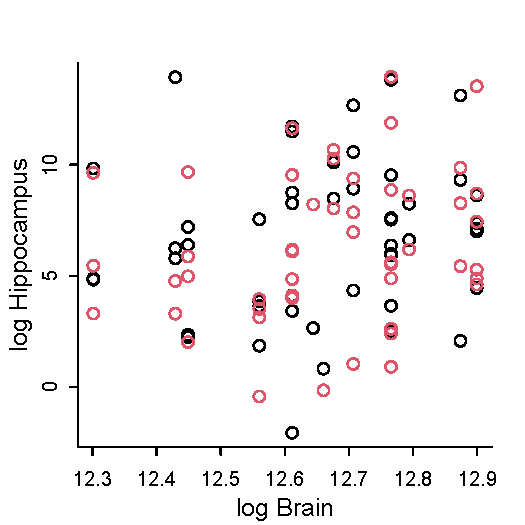
\includegraphics[scale=0.7]{fig_prior_pred_m1.pdf}
\end{center}

The prior predictive distribution for these priors is surely too wide---it includes many very large hippocampus volumes. However it contains no bias for a difference between wild and captive, and the wide priors help us to notice model misspecification when it is present. The code base contains a module for reproducing and plotting this prior predictive distribution.


\subsection{Growth model}
x

Hippocampus volume $H$ is necessarily an age-specific proportion $p$ of total brain volume $B$.
\begin{align}
H = p_A B
\end{align}
On the log scale, which we'll use for modeling, this is:
\begin{align*}
\log H = \log p_A + \log B
\end{align*}
The proportion $p_A$ could increase or decrease with age, because while the volume of the hippocampus increases with age, and the volume of the brain increases with age, the relative volume could increase or decrease.


\subsection{Dimensionless analysis}

Often it is revealing to divide out all measurement scales and express the relations among measurements as dimensionless ratios.


\section{Implementation}

x


%%%%%%%%%%%%%%%%%%%%%%%
\clearpage
\bibliographystyle{apalike} 
\bibliography{repertoire_refs}

\end{document}








